\documentclass[12pt,a4paper]{scrartcl}

\usepackage[ngerman]{babel}
\usepackage[ansinew]{inputenc}

\usepackage{float}

\usepackage[pdftex]{graphicx}
\usepackage{latexsym}
\usepackage{amsmath,amssymb,amsthm}
\usepackage[linesnumbered,ruled]{algorithm2e}
\usepackage[table]{xcolor}
\usepackage{subfig}
\usepackage{listingsutf8}

\lstset{ % General setup for the package
	language=Java,
	basicstyle=\small\sffamily,
	numbers=left,
	numberstyle=\tiny,
	frame=tb,
	tabsize=2,
	columns=fixed,
	showstringspaces=false,
	showtabs=false,
	keepspaces,
	commentstyle=\color{red},
	keywordstyle=\color{blue}
}

% Abstand obere Blattkante zur Kopfzeile ist 2.54cm - 15mm
\setlength{\topmargin}{-15mm}


\begin{document}
	
	% Keine Seitenzahlen im Vorspann
	\pagestyle{empty}
	% Titelblatt der Arbeit
	\begin{titlepage}
		
		\begin{center}
			\vspace*{2cm} 
		\end{center}
		
		\begin{center} \large 
			
			Praxisprojekt
			\vspace*{1cm}
			
			{\huge Half-Edge Mesh f\"ur Unity3D}
			\vspace*{1.5cm}
			
			Erstellt von:\\
			Yannick Dittmar\\Studiengang: Allgemeine Informatik\\ Matrikelnummer: 11117676
			
			\vspace*{1.5cm}
			
			Datum der Abgabe: xx.xx.xxxx
			\vspace*{1.5cm}
			
			
			Betreuung: Dennis Buderus \\[1cm]
			Technische Hochschule K\"oln\\
			Fakult\"at f\"ur Informatik und Ingenieurswissenschaften
		\end{center}
	\end{titlepage}

\pagestyle{headings}

\section{Einleitung}
In der Computergrafik werden dreidimensionale Modelle als Polygonen-Netz (Polygonal Mesh) dargestellt, um diese auf einem zweidimensionalen Bildschirm darzustellen. Die Oberfl\"ache eines Modells wird dabei mit Hilfe von Polygonen angen\"ahert. H\"aufig werden daf\"ur Dreiecks-Netze (Triangle Mesh) verwendet, wobei die Fl\"achen mit Dreiecken nachmodelliert werden, siehe Abbildung \ref{fig:dolphintrianglemesh}. 
\\Ein solches Netz besteht aus den Eckpunkten der einzelnen Dreiecke, den Vertices. Diese werden durch Kanten (Edges) verbunden und bilden damit die Polygonalfl\"achen, auch Faces genannt. 

\begin{figure}[h]
	\centering
	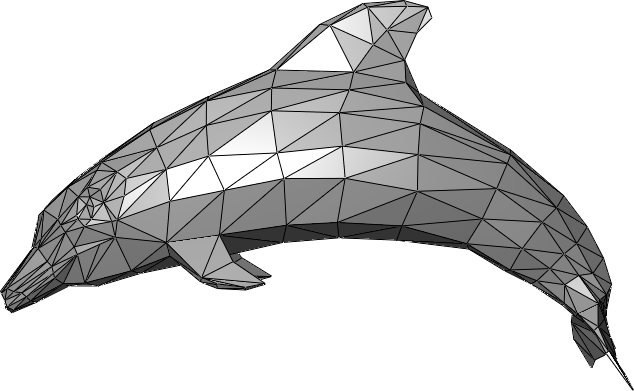
\includegraphics[width=0.7\linewidth]{Images/Dolphin_triangle_mesh}
	\caption[Beispiel eines Polygonen-Netzes]{Beispiel eines Dreiecks-Polygonen-Netz, von \cite{WikipediaDolphin1}}
	\label{fig:dolphintrianglemesh}
\end{figure}

\section{Unity}
Unity ist eine Spiele-Engine mit eingebauter Entwicklungsumgebung f\"ur 2D-, 3D- und VR-Spiele/-Simulationen. Die Engine kommt mit einem eigenen Editor, in welchem diverse Szenarien erstellt und bearbeitet werden k\"onnen. Des Weiteren unterst\"utzt Unity selbst programmierte Scripte auf der Grundlage von C\#.
\subsection{Meshes in Unity}
Unity bietet die M\"oglichkeit, mit Hilfe von selbstgeschriebenen Scripten eigene 3D-Modelle zur Laufzeit erstellen zu lassen. Daf\"ur stellt Unity ein eigenes Mesh-System zur Verf\"ugung, basierend auf Dreiecksnetzen, die \textit{UnityEngine.Mesh}-Klasse. Damit diese ein Mesh rendern kann, erwartet das Mesh ein \textit{UnityEngine.Vector3}-Array f\"ur die Vertices, wobei ein \textit{Vector3} einen Punkt im dreidimensionalen Raum darstellt und ein \textit{int}-Array, das die Reihenfolge der Vertices (\"uber die Indices der Vertices) f\"ur die Dreiecke festlegt.   
\\
Der folgende Code zeigt beispielhaft, wie ein Unity-Mesh erzeugt werden kann:
\begin{lstlisting}
public void CreateMesh()
{
	//--- Der Vollstaendigkeit halber vorhanden
	meshFilter = gameObject.GetComponent<MeshFilter>();
	if (meshFilter == null)
		meshFilter = gameObject.AddComponent<MeshFilter>();

	//--- vom MeshFilter zum Mesh
	mesh = meshFilter.sharedMesh;
	if (mesh == null)
		mesh = new Mesh { name = "Quad" };

	//--- MeshRenderer holen
	meshRenderer = this.gameObject.GetComponent<MeshRenderer>();
	if (meshRenderer == null)
		meshRenderer = gameObject.AddComponent<MeshRenderer>();

	//--- Mesh zusammenstellen
	//--- Vertices/Points
	var P0 = new Vector3(0, 0, 0);
	var P1 = new Vector3(0, 1, 0);
	var P2 = new Vector3(1, 0, 0);
	var P3 = new Vector3(1, 1, 0);
	
	var verticies = new List<Vector3> { P0, P1, P2, P3 };

	//--- Triangles
	var triangles = new List<int>();

	triangles.Add(0);
	triangles.Add(1);
	triangles.Add(2);
	triangles.Add(2);
	triangles.Add(1);
	triangles.Add(3);

	//--- Mesh befuellen
	mesh.Clear();
	//--- Vertices zuweisen
	mesh.vertices = verticies.ToArray();
	//--- Triangles zuweisen
	mesh.triangles = triangles.ToArray();
	//--- Mesh dem MeshFilter zuweisen
	meshFilter.sharedMesh = mesh;
}
\end{lstlisting}

Und liefert folgendes Ergebnis:
\begin{figure}[h]
	\centering
	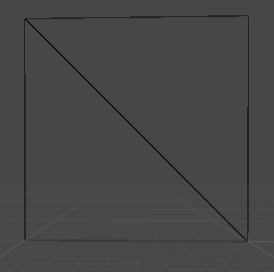
\includegraphics[width=0.35\linewidth]{Images/UnityQuadWireframe}
	\caption[Die Wireframeansicht des erstellten Meshes]{Die Wireframeansicht des erstellten Meshes im Unity Editor}
	\label{fig:unityquadwireframe}
\end{figure}

\subsection{Nachteile von Unity-Meshes}
Die Vorteile bei dieser Herangehensweise sind, dass die von Unity verwendeten Netze auch bei gr\"o{\ss}eren Netzen vergleichsweise wenig Speicherplatz ben\"otigen, da dieser Ansatz auf eine direkte Repr\"asentation von Faces und Edges verzichtet. Daraus ergeben sich einige Nachteile. Durch die fehlende Referenz auf die Polygonenfl\"achen sind Operationen auf Face-Ebene, wie eine Nachbarsuche, Abfragen auf alle Punkte Kanten oder die Unterteilung einzelner Polygonen in kleinere Einheiten (auch ,,Subdivision'' genannt), sehr Zeitintensiv, weshalb sich solche F\"alle nicht f\"ur Echtzeitanwendungen eignen. Des Weiteren stehen die Vertices im Unity-Mesh in keinem topographischen Zusammenhang, wodurch eine Iteration \"uber das gesamte Netz erschwert wird, um beispielsweise zusammenh\"angende Punkte zu bearbeiten.
	
\section{Half-Edge-Mesh}
Um die oben genannten Problemstellungen zu l\"osen, gibt es andere Ans\"atze Polygonalnetze zu realisieren. Einer dieser L\"osungen ist das Konzept der Half-Edge-Meshes. Ein solches Mesh besteht aus folgenden Komponenten: 
\begin{itemize}
	\item eine Liste von Vertices
	\item eine Liste von Faces
	\item eine Liste von Half-Edges.
\end{itemize}

Die Vertices sind, wie im Unity-Mesh auch, die Eckpunkte der Polygonen. Die Vertices werden mithilfe von Half-Edges miteinander verbunden. 

\subsection{Vertex}
Ein Vertex ist ein Punkt im dreidimensionalen Raum und ist wie beim einfachen Mesh der Eckpunkt f\"ur die Polygonen. Neben einem \textit{Vector3} f\"ur die Position des Vertex wird eine Referenz auf eine ausgehende Half-Edge, sowie der Index des Vertex ben\"otigt.
\\
\begin{lstlisting}
public class Vertex
{
	public event EventHandler PositionChangedEvent;
	
	public Vertex(Vector3 point)
	{
		Point = point;
		Index = -1;
	}

	public Vertex(Vector3 point, int index)
	{
		Point = point;
		Index = index;
	}

	public Vertex(float x, float y, float z) : this(new Vector3(x, y, z))
	{ }

	public Vertex(float x, float y, float z, int index) : this(new Vector3(x, y, z), index)
	{ }

	/// <summary>
	/// The Index of the Vertex
	/// </summary>
	public int Index { get; set; }

	private Vector3 _point;
	/// <summary>
	/// The Point
	/// </summary>
	public Vector3 Point
	{
		get => _point;
		set
		{
			_point = value;
			PositionChangedEvent?.Invoke(this, EventArgs.Empty);
		}
	}

	/// <summary>
	/// The Outgoing HalfEdge
	/// </summary>
	public HalfEdge HalfEdge { get; set; }
}
\end{lstlisting}

\subsection{Face}
Ein Objekt der Klasse Face repr\"asentiert die Faces des Meshs, die \"uber die Vertices aufgespannt werden. Dabei besitzt eine Face nur die Referenz auf eine der anliegenden Half-Edges um das Traversieren und Bearbeiten des Netzes auf Face-Ebene zu erm\"oglichen. Die Face-Klasse ist wie folgt aufgebaut:
\begin{lstlisting}
public class Face
{
	public Face(HalfEdge halfEdge)
	{
		HalfEdge = halfEdge;
	}

	/// <summary>
	/// A bonding HalfEdge
	/// </summary>
	public HalfEdge HalfEdge { get; set; }
}
\end{lstlisting}

\subsection{Half-Edge}
Die Half-Edge Klasse ist die wichtigste Komponente f\"ur das Half-Edge-Mesh. Sie stellt alle Teile in Beziehung zueinander. Zu bemerken ist, dass ein Half-Edge-Mesh keine explizite Modellierung von Edges hat. Eine Edge wird implizit durch zwei Half-Edges abgebildet. Jede Half-Edge besitzt eine Referenz auf ihre gegen\"uberliegende Half-Edge, sowie auf die ihr Nachfolgende. Zudem referenziert jede Half-Edge den Vertex, aus dem sie hervorgeht und die Face, die sie einschlie{\ss}t. 
\begin{lstlisting}
public class HalfEdge
{
	public HalfEdge(Vertex outgoing, Face face, HalfEdge next)
	{
		OutgoingPoint = outgoing;
		Face = face;
		Next = next;
		Index = -1;
	}
	
	public HalfEdge(Vertex outgoing, Face face, HalfEdge next, int index)
	{
		OutgoingPoint = outgoing;
		Face = face;
		Next = next;
		Index = index;
	}
	
	public int Index { get; set; }
	
	/// <summary>
	/// The Vertex the HalfEdge comes from
	/// </summary>
	public Vertex OutgoingPoint { get; set; }
	
	/// <summary>
	/// The next HalfEdge, Counter Clockwise
	/// </summary>
	public HalfEdge Next { get; set; }
	
	/// <summary>
	/// The opposing HalfEdge
	/// </summary>
	public HalfEdge Opposing { get; set; }
	
	/// <summary>
	/// The face of the HalfEdge
	/// </summary>
	public Face Face { get; set; }
	
	/// <summary>
	/// Getter for the previous HalfEdge, for easier access 
	/// (this.Next.Next)
	/// </summary>
	public HalfEdge Previous => Next.Next;
	
	/// <summary>
	/// Getter for the EndPoint of this HalfEdge, for easier access (this.Next.OutgoingPoint)
	/// </summary>
	public Vertex EndPoint => Next.OutgoingPoint;
}
\end{lstlisting} 


\newpage
\bibliography{Hauptdokument}
\bibliographystyle{alpha}

\end{document}